\documentclass[11pt]{article}
\usepackage{classTools}
\graphicspath{ {./photos/} }
\begin{document}

\psHeader{6}{Wed Oct. 26, 2022 (11:59pm)}

\textbf{Your name: Cory Zimmerman}

\textbf{Collaborators: None}

\textbf{No. of late days used on previous psets: 0}

\textbf{No. of late days used after including this pset: 0}

\begin{enumerate}
 \item (Matching Algorithms) 
 One practical application of matching algorithms is planning logistics, like in the following example from (fictional) ridesharing service Lyber in (real) New York City's Times Square.  When a customer books a Lyber ride, the ride request is sent to a Lyber server and combined with others to create a schematic 
 like the one drawn in the map below:
\begin{figure}[H]
    \centering
    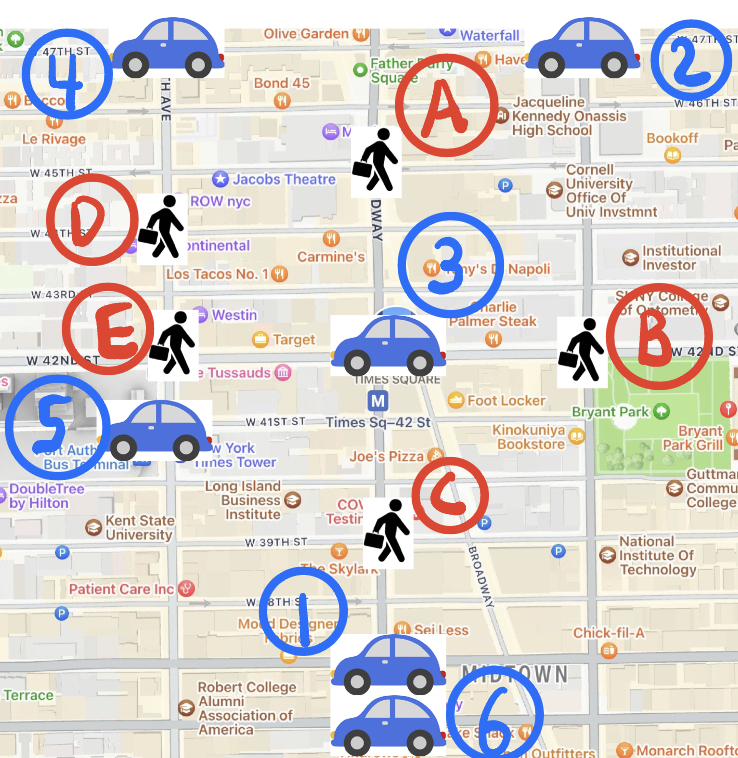
\includegraphics[width=0.87\textwidth]{NYC-map-zoomed-light.jpeg}
    \label{fig:travel_time_graph}
\end{figure}
Given a schematic like this, Lyber's goal is to serve as many customers (labeled A--E in the map) as possible, by assigning each one to a driver (labeled 1--6 in the map). For simplicity, each customer and driver is at an intersection, and assume driving between adjacent streets (vertical segment) takes 30 seconds, and driving between adjacent avenues (horizontal segments) takes 1 minute. However, the one twist is that they want to make sure that \textit{no customer is waiting for longer than 2 minutes}.  They also do not want to assign a driver to more than one customer at once, since serving a single customer can take more than 2 minutes.

    \begin{enumerate}
    \item To perform the assignment, they reduce to Maximum Matching in bipartite graphs.  Draw a bipartite graph corresponding to the drivers and customers in the map above.
     \begin{quote}
        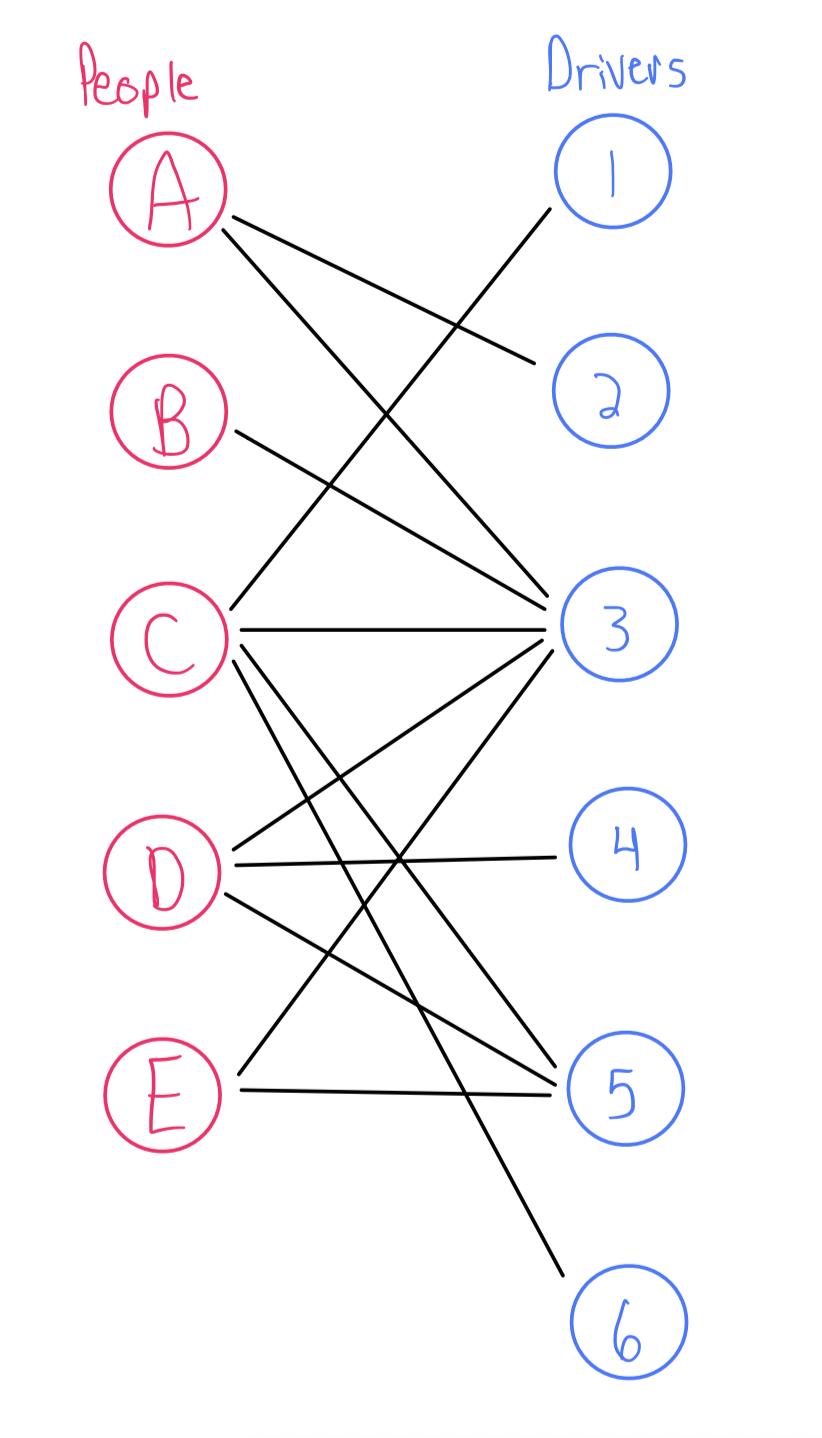
\includegraphics[scale=0.4]{photos/q1a.png}
     \end{quote}

    
    \item The Lyber app first prioritizes customers on Broadway, so they initially assign customer $A$ to driver 3 and customer $C$ to driver 5. Using the algorithm from class, find a \textit{maximum matching} in the bipartite matching graph you've drawn, starting from the initial matching of $A$ to 3 and $C$ to 5. Draw pictures showing the sequence of matchings and augmenting paths you find. (No need to break down the steps of the algorithm to find the augmenting paths.)
     \begin{quote}
        \color{purple}
        \hspace*{-1.5in}
        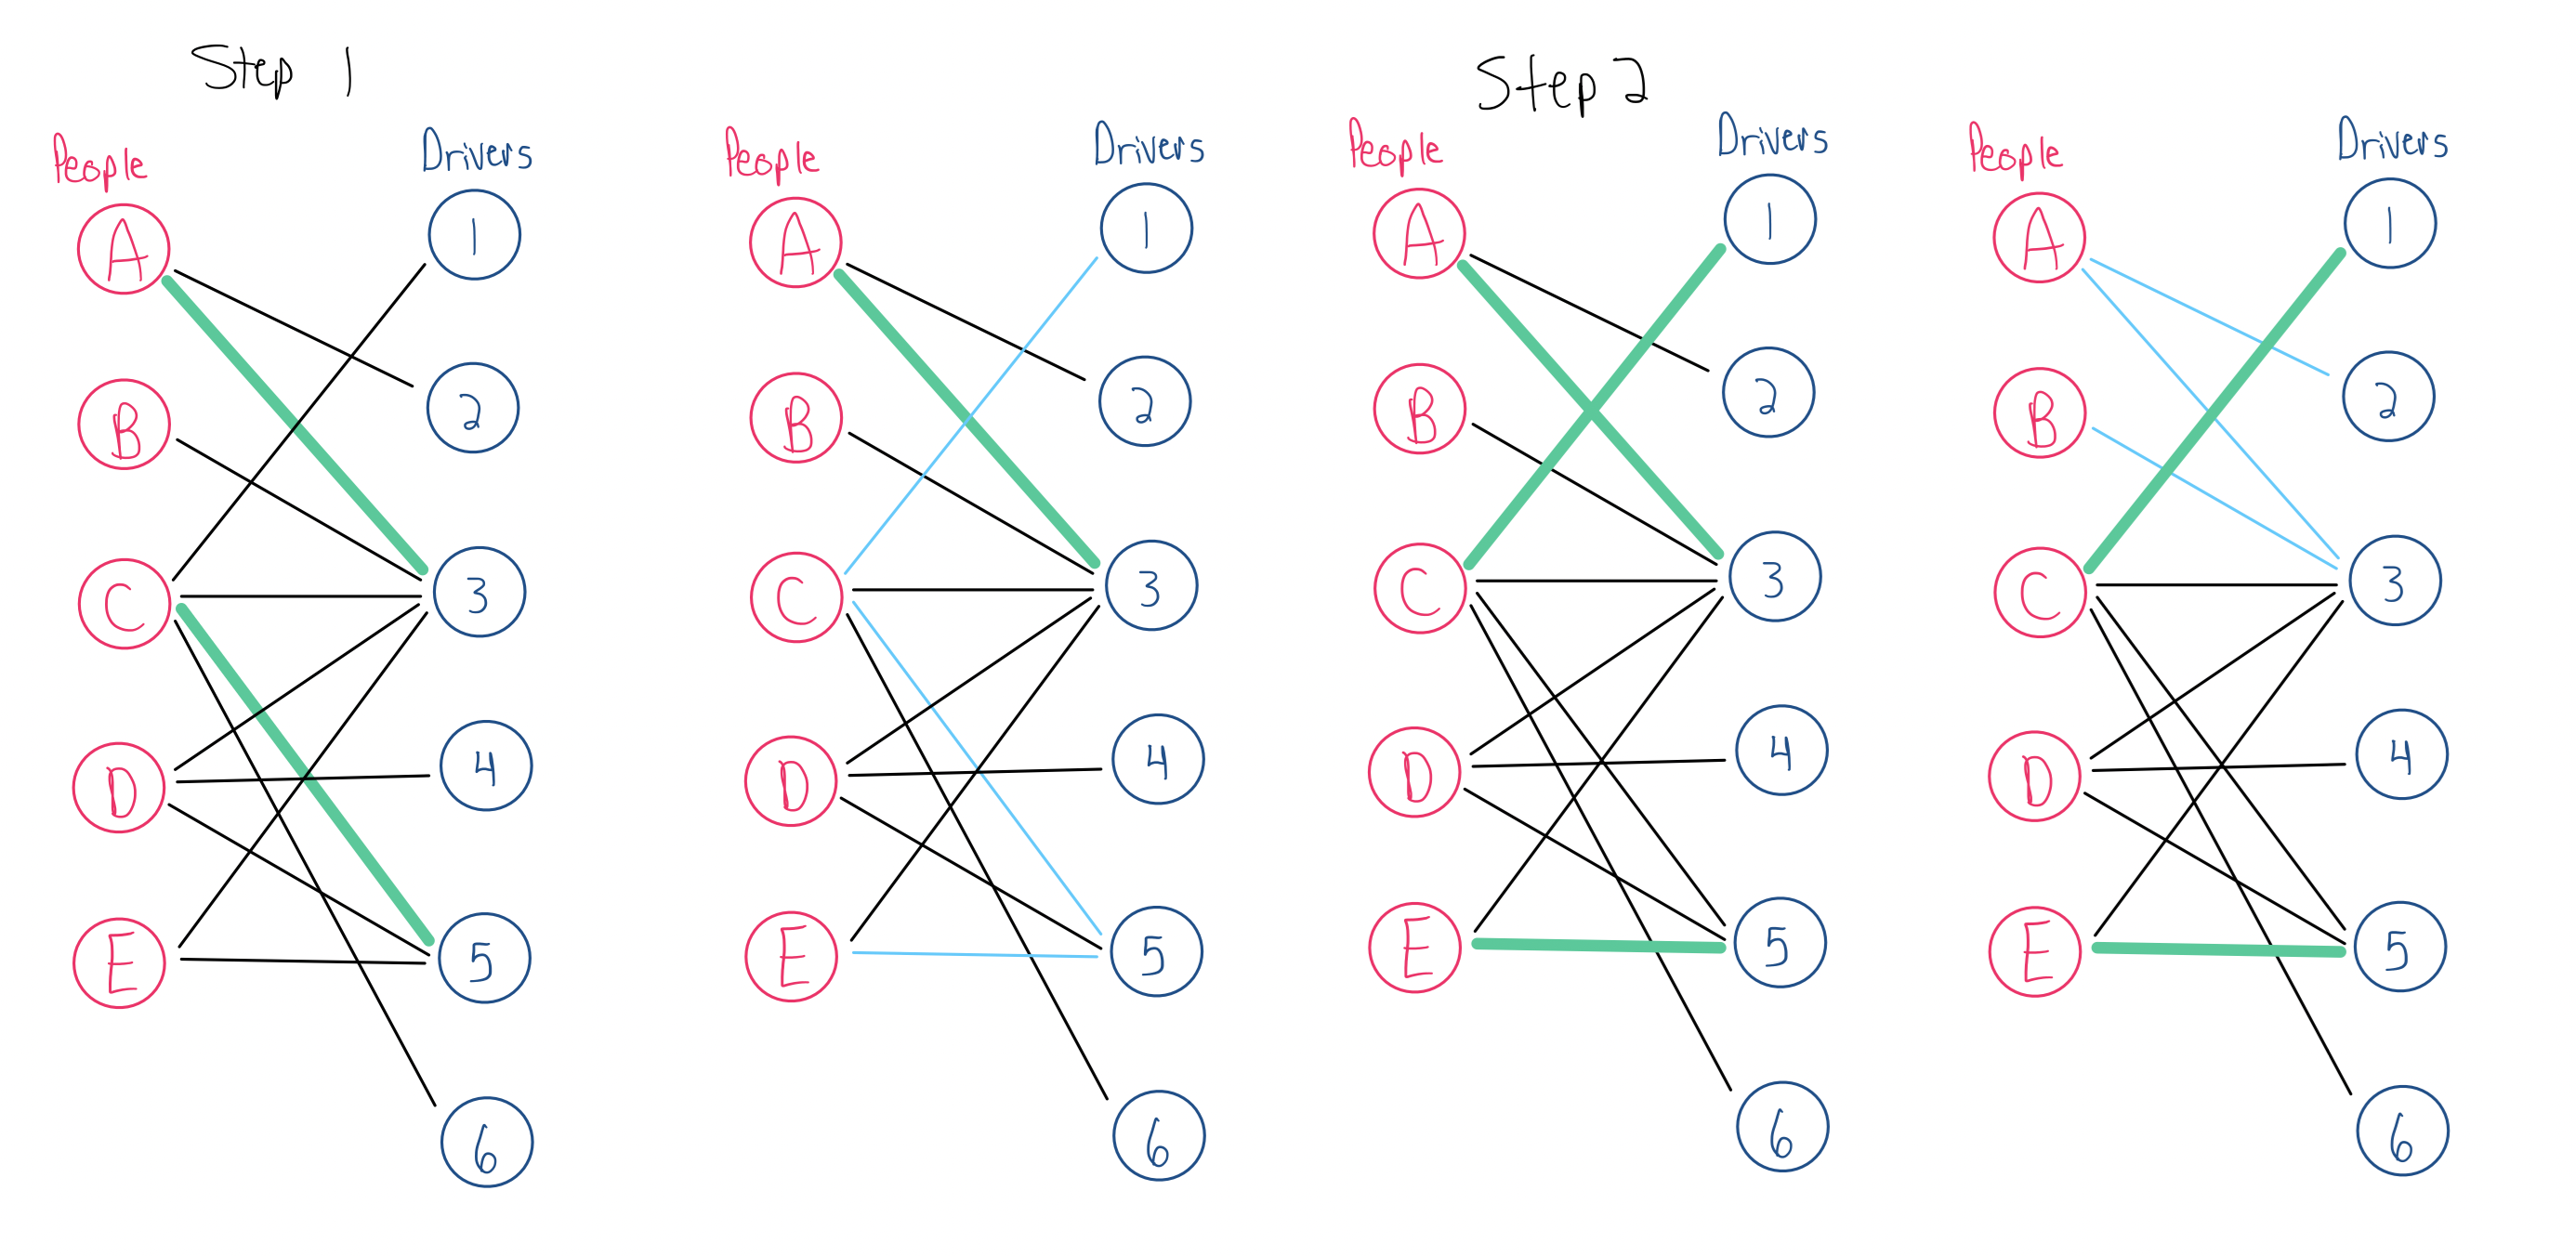
\includegraphics[scale=0.4]{photos/q1b 1.png}
        \hspace*{-1.5in}
        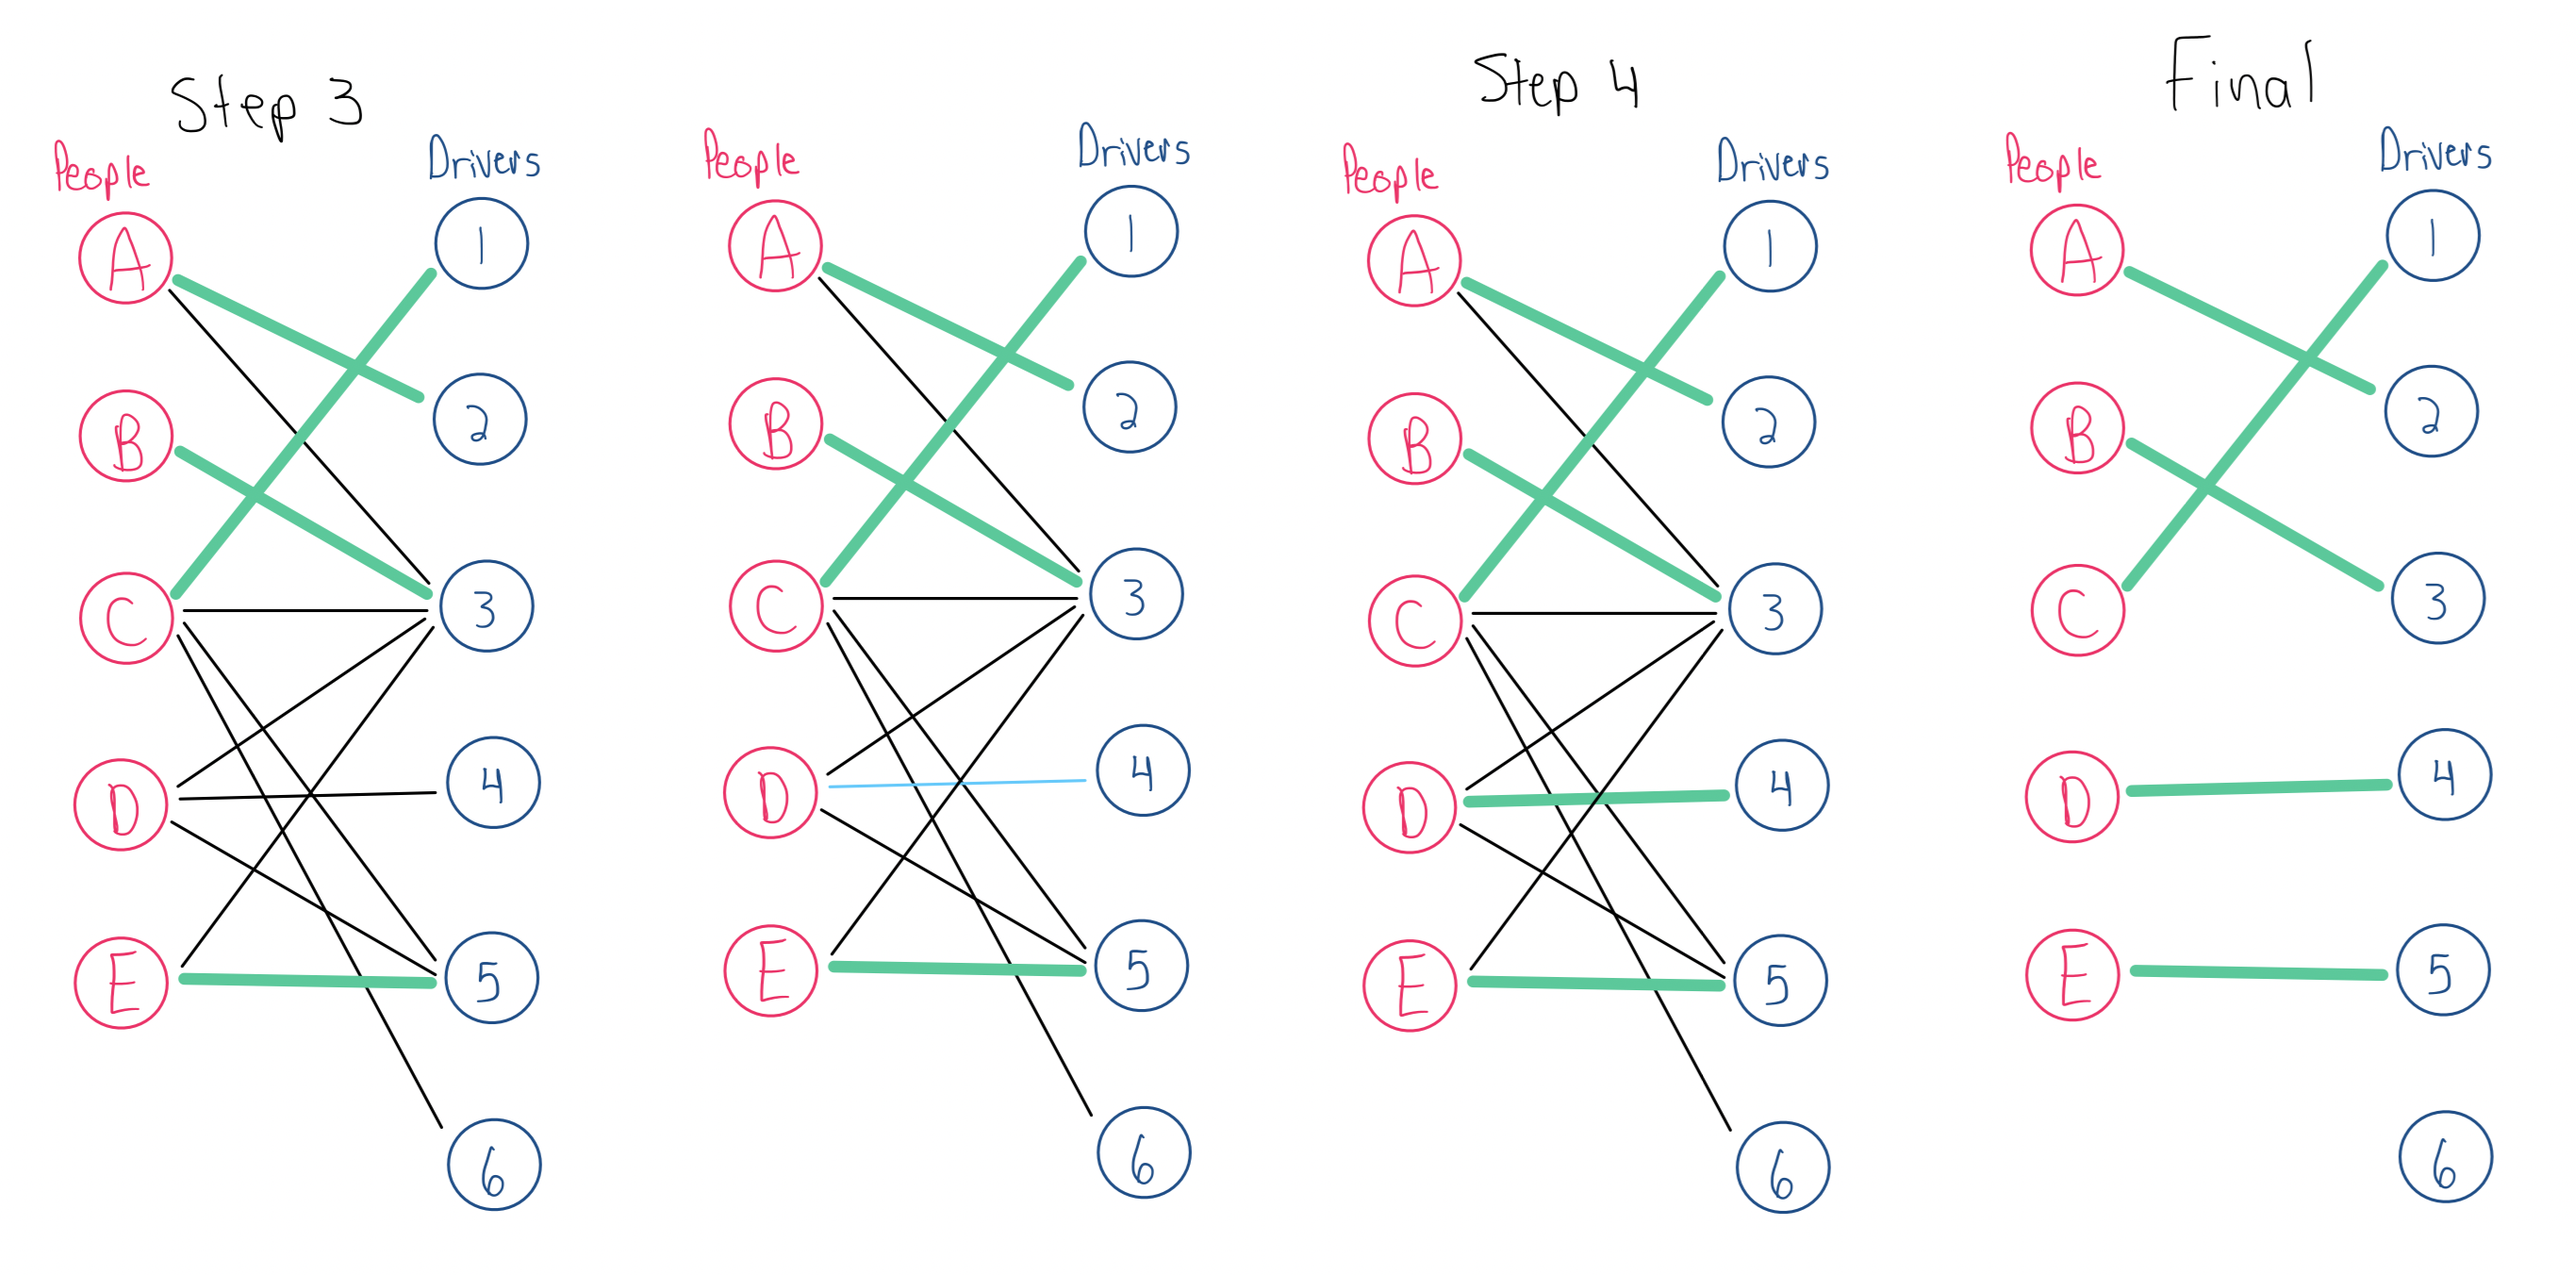
\includegraphics[scale=0.4]{photos/q1b 2.png}
        \\ \\ 

        Black lines indicate ordinary edges. Light blue lines represent augmenting paths. Thick green lines represent a matching.
     \end{quote}

    \item The Lyber app also allows users to schedule trips in advance. One Lyber driver receives the following pre-programmed trips scheduled by 4 different users (all of them need multiple rides on the same day):
    \begin{itemize}
        \item User A: one trip from 10 to 10:29, another from 11 to 11:59, another from 12:15 to 12:29, and another from 13 to 13:29.
        \item User B: one trip from 10:15 to 11:14, another from 11:30 to 12:14, and another from 12:45 to 13:14.
        \item User C: one trip from 10:30 to 11:44, another from 12:30 to 12:59, and another from 13:15 to 13:44.
        \item User D: one trip from 10 to 10:44, another from 11:15 to 11:29, another from 12 to 12:44, and another from 13:30 to 13:59.
    \end{itemize}
    The Lyber driver wants to maximize the total number of different rides, because they earn a fixed rate per ride. (The driver is \textit{not} trying to maximize the driving time). 
    We also assume for simplicity that the driver needs no time to move between different rides (i.e., it is possible that one ride finishes at 10:29 and the next one starts immediately at 10:30). 
    Use a greedy algorithm that we saw in class to find a maximum-sized set of non-conflicting rides.  State which algorithm you are using, how you are applying it to this ride-selection problem, and write down the order in which the greedy algorithm selects the rides in the solution. 

    \begin{quote}
        \color{purple}
        Using the GreedyAlgorithmScheduling algorithm from class, I can sort the inputs by increasing order of end time and iteratively select the interval with the earliest end time that doesn't intersect any other chosen interval. To make the process of sorting and selecting more visual, I drew a picture of this decision process similar to the one Adam drew in class: \newline 

    \hspace*{-1.25in}
    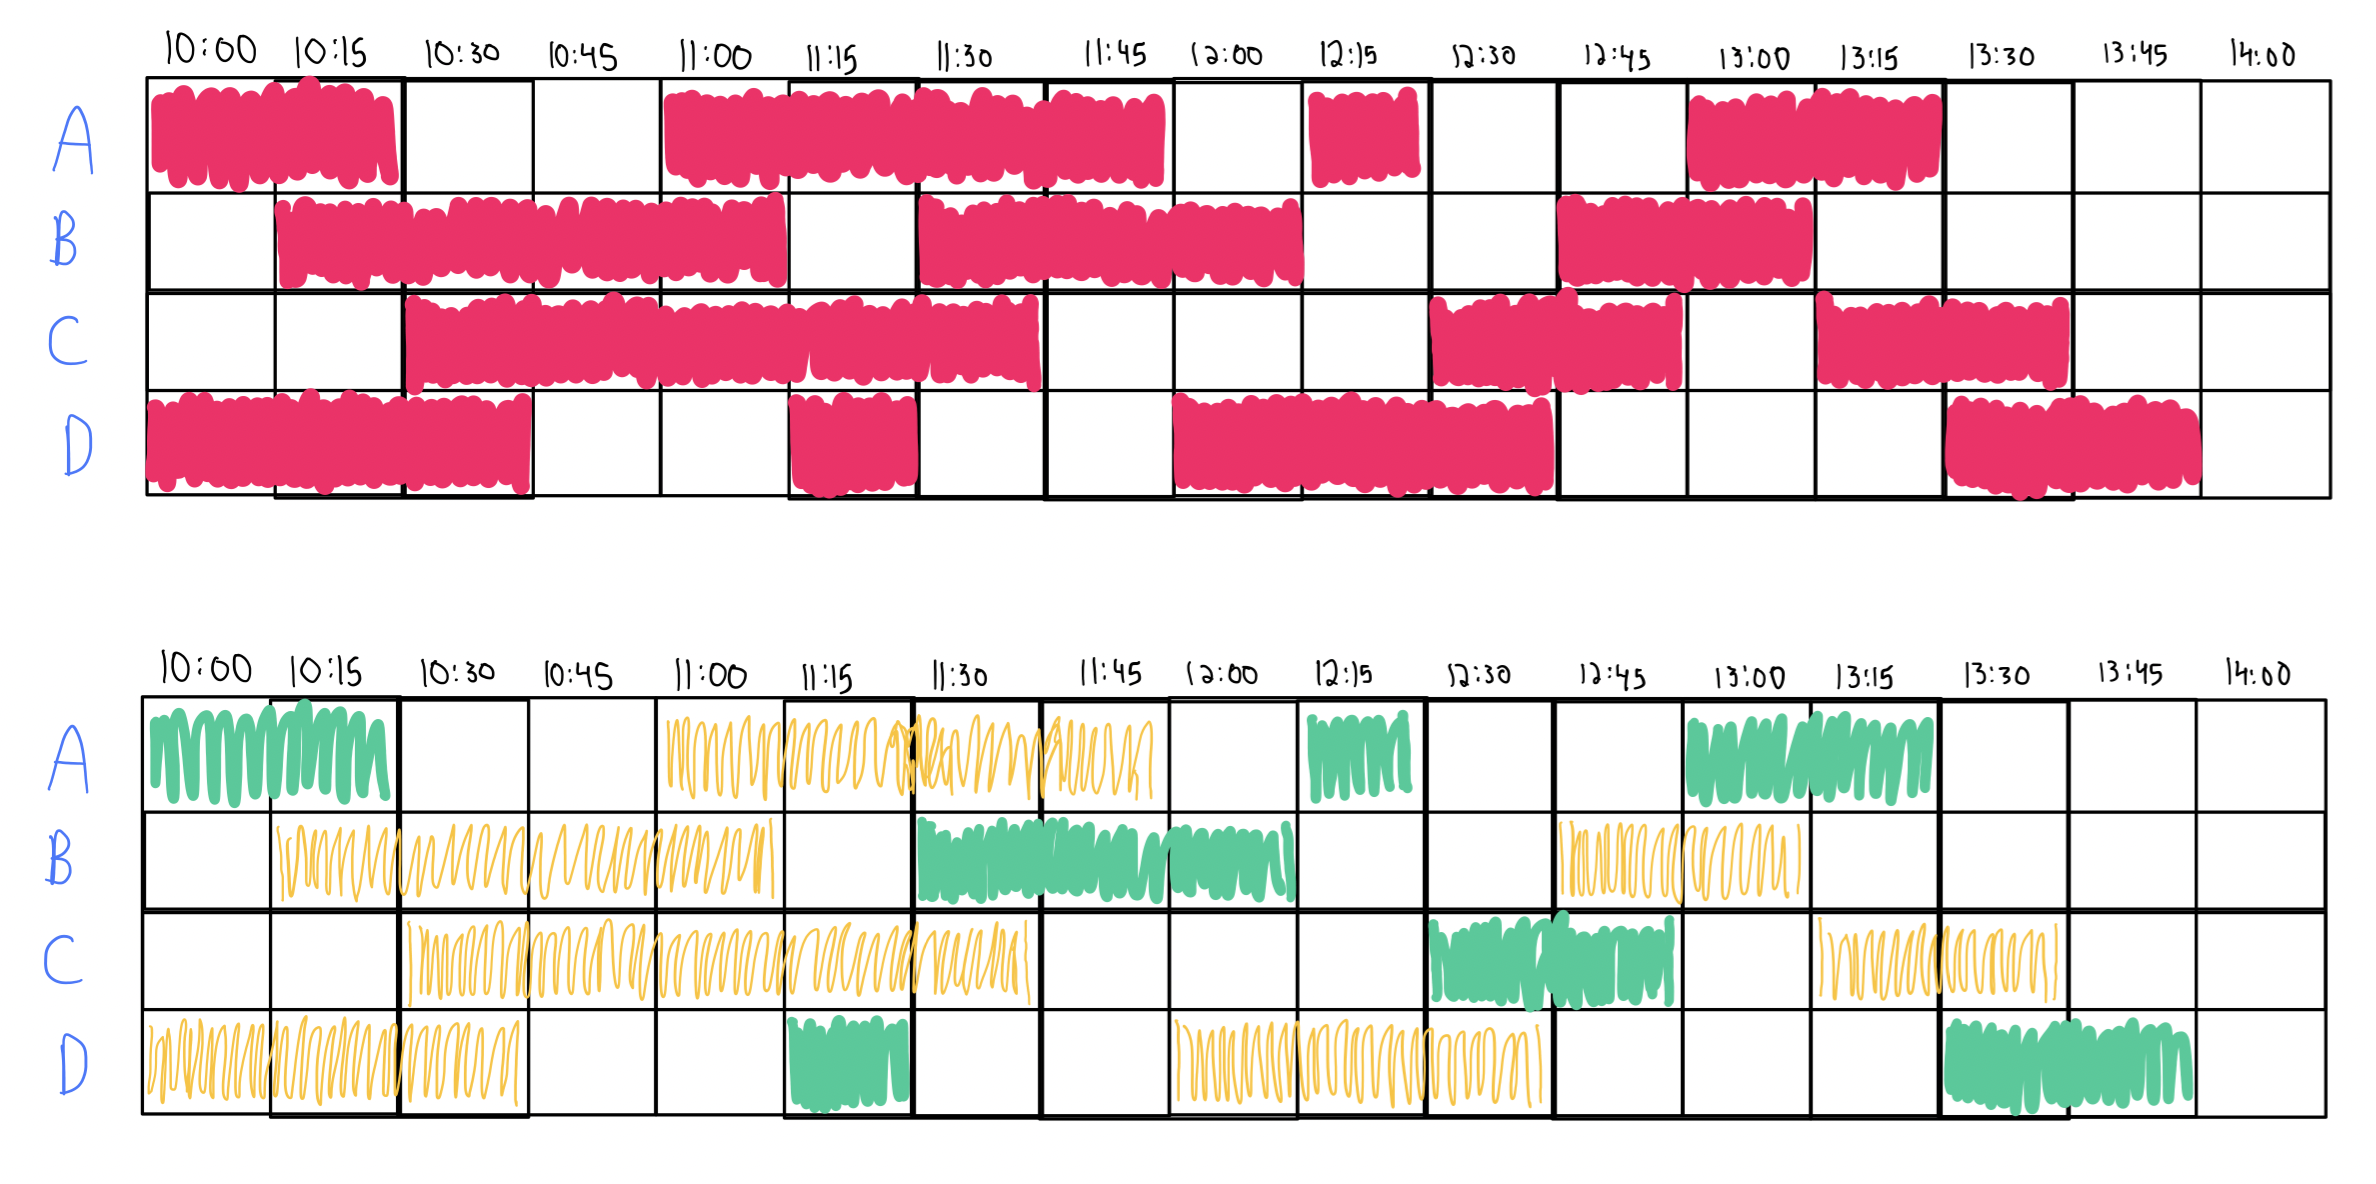
\includegraphics[scale=0.4]{q1d.png}

    In the picture above, the initial intervals are all pink. Selected intervals are green, and intersecting intervals are gold. This was the selection process: 
    \begin{itemize}
        \item User A's trip from 10 to 10:29 finishes first, choose that. Accepting this trip invalidates intersecting trips from users B and D.
        \item Next, User D's trip from 11:15 to 11:29 finishes before any other trip. So, choose that and toss intersecting trips from users C and A.
        \item After that, User B's trip from 11:30 to 12:14 finishes first, so choose that and cross off the 12:00 trip from user D.
        \item Then, the 12:15 to 12:29 trip from User A finishes first, so take that.
        \item User C's trip from 12:30 to 12:59 finishes earliest, so take that next, skipping User B's trip at 12:45.
        \item At 13:00, take user A's trip until 13:29, skipping the 13:15 trip from User C.
        \item Finally, take User D's trip from 13:30 to 13:59.
    \end{itemize}
    By sorting intervals by end time and choosing greedily based on end time, the algorithm yields seven viable trips in this time window. By Theorem 2.1 from class, this is an optimal solution solved in time $O(n \log n)$.
    \end{quote}
    \end{enumerate}

 \item (EthiCS Reflection)
Suppose there are two patients in need of an immediate kidney transplant, but only one donor is currently available. The donor’s kidney is compatible with both patients. Patient A starts at 30 QALYs and is expected to live 6 additional years as a result of the transplant. Patient B starts at 45 QALYs, and is expected to live 10 additional years as a result of the transplant. {\em All else being equal}, \underline{\textbf{which patient should the kidney go to, and why?}} Your response should take the form of a short paragraph (3-4 sentence) reflection. {\em In explaining your ethical reasoning about the case, be sure to draw on at least one concept discussed in class.}

\begin{quote}
    \color{purple}
    Such a decision is never easy, but I generally believe patient B should get the kidney. This follows the utilitarian approach mentioned in the presentation. While it seems harsh, I see it as a more applicable standard than something like Prioritarianism, which sounded very subjective. The needs-based approach also does not appeal to me because it seems prone to wasting resources. It's harsh, but, say, for example, someone might only live for a few months after receiving a transplant. It's hard to justify someone else's potential years of life on a few months for someone else. I see utilitarianism as a reasonable standard by which to allocate a scarce resource like organs among without depending on very emotionally and politically charged arguments about whose time on earth is worth more. This assertion, however, does rest on the assumption QALYs can be objectively assessed and the system cannot be gamed.
\end{quote}
 
 \item (Vertex-Weighted Matching)
        For a graph $G=(V,E)$ and a subset $F\subseteq E$, 
        let $V(F)$ denote the set $\bigcup_{f \in F}f$ of 
        vertices that are an endpoint of at least one edge in $F$.
        \begin{enumerate}
        \item Prove that if $G=(V,E)$ is a graph and $M\subseteq E$ is a matching in $G$, then there is a maximum-size matching $M'$ such that $V(M)\subseteq V(M')$.  (Hint: consider constructing a maximum matching via augmenting paths, but starting with $M_0=M$ rather than $M_0=\emptyset$. What can you say about the $V(M_i)$'s?) \label{part:monotonicity}

        \begin{quote}
            \color{purple}
            Let $M$ be some valid matching of the vertices in a graph $G$. To construct $M'$, begin by letting $M'$ equal $M$. Then, search for augmenting paths in $M'$ until none more are found. For each augmenting path that's found, flip the edges of the augmenting path such that those previously in $M'$ are dropped and those new to $M'$ are added. This process is guaranteed to increase the size of $M'$ by one during each iteration due to a counting argument asserted in the lecture notes. By Berge's Theorem, this process will continue until $M'$ is a maximum size matching. \\ 

            Because $M'$ is initialized as equal to $M$, every vertex in $M$ is initially in $M'$. At each step of the algorithm, the augmenting path is definitionally guaranteed to begin and end at vertices not belonging to $M'$. Within the augmenting path, the edges initially in $M$ might be rotated out of $M'$ due to the flipping process, but the augmenting path guarantees that an edge lost on one side of an intermediate vertex is an edge gained on another side. Because of this, no flip or expansion of the graph causes the vertices initially in $M$ to be dropped. So, by the end, every vertex in $M$ is also in $M'$. This makes $V(M)$ a subset of $V(M')$.
        \end{quote}

        \item   In the Embedded EthiCS module, we saw how simply maximizing the {\em size} of a matching may not always be the right objective.  Thus, it is natural to consider weighted versions of the matching problem. Suppose 
        we consider vertex-weighted graphs $G = (V,E,w)$, $w$ is an array specifying a nonnegative edge weight $w(v)$ for every $v\in V$.  (For example, the weight assigned to a patient might correspond to the number of extra years of life they would gain from a donation.)
          The goal of the {\em vertex-weighted maximum matching problem} is to find a matching $M$ maximizing its {\em total weight} $$w(M) = \sum_{\{u,v\}\in M} (w(u)+w(v)).$$
        (This corresponds to the utilitarian objective discussed in Embedded EthiCS module.)
        Using Part~\ref{part:monotonicity}, prove that every graph $G$ has a matching $M^*$ that simultaneously maximizes both total weight and size.  That is, for every matching $M$ in $G$, we have
        both $w(M)\leq w(M^*)$ and $|M|\leq |M^*|$.

        \begin{quote}
            \color{purple}
            Assert the existence of some MaximumSizeMatching algorithm which returns a matching of maximum size from the given graph (the same algorithm used in proof $3a$). Use this algorithm to check every possible combination of vertices among the maximum size matchings of the graph. Let $M^*$ be the maximum size matching with greatest weight such that any maximum size matching $M'$ from graph $G$ has weight less than or equal to the weight of $M^*$. \\

            Let $M$ represent any possible matching from the input graph. By definition of a maximum size matching, the size of $M^*$ is greater than or equal to the size of $M$ such that $|M|\leq |M^*|$. The weight of $M$ is $w(M)$. By proof $3a$, there exists some maximum matching $M'$ such that every vertex in $M$ is also in $M'$. Because vertex weights are nonnegative, the weight of $M'$ is the weight of the vertices in $M$ plus the weight of additionally-added vertices. This implies $w(M) \leq w(M')$. Because $M^*$ was chosen to be the maximum size matching of weight greater than or equal to every other maximum size matching, it must be the case that $w(M) \leq w(M') \leq w(M^*)$, which simplifies to $w(M) \leq w(M^*)$. \\

            Thus, there must exist some maximum matching of maximum weight $M^*$ such that $w(M)\leq w(M^*)$ and $|M|\leq |M^*|$ for any possible matching $M$ in the input graph.
        \end{quote}

        \item (optional\footnote{This problem won't make a difference between N, L, R-, and R grades. As this problem is purely extra credit, course staff will deprioritize questions about this problem at office hours and on Ed.}) Explain why the same holds for the maximin objective discussed in the Embedded EthiCS module.  That is, there is always a matching $M$ that simultaneously maximizes the maximin objective and $|M|$. 
        \end{enumerate}
        

\item (Edge-Weighted Bipartite Matching) 
  Instead of considering vertex weights, we could instead study matching on
{\em edge-weighted} bipartite graphs $G = (V,E,w)$, where $w$ is an array specifying a nonnegative edge weight $w(e)$ for every $e\in E$.  

   The goal of the {\em edge-weighted maximum matching problem} is to find a matching $M$ maximizing $$w(M) = \sum_{e\in M} w(e).$$
   \begin{enumerate}
    \item Construct an edge-weighted bipartite graph $G = (V,E,w)$ such that there is no matching $M$ in $G$ that simultaneously maximizes the weight $w(M)$ and the size $|M|$.  Thus, there can be an inherent tension between these two objectives. 
   \begin{quote}
    \color{purple}
        \hspace*{-1.25in}
        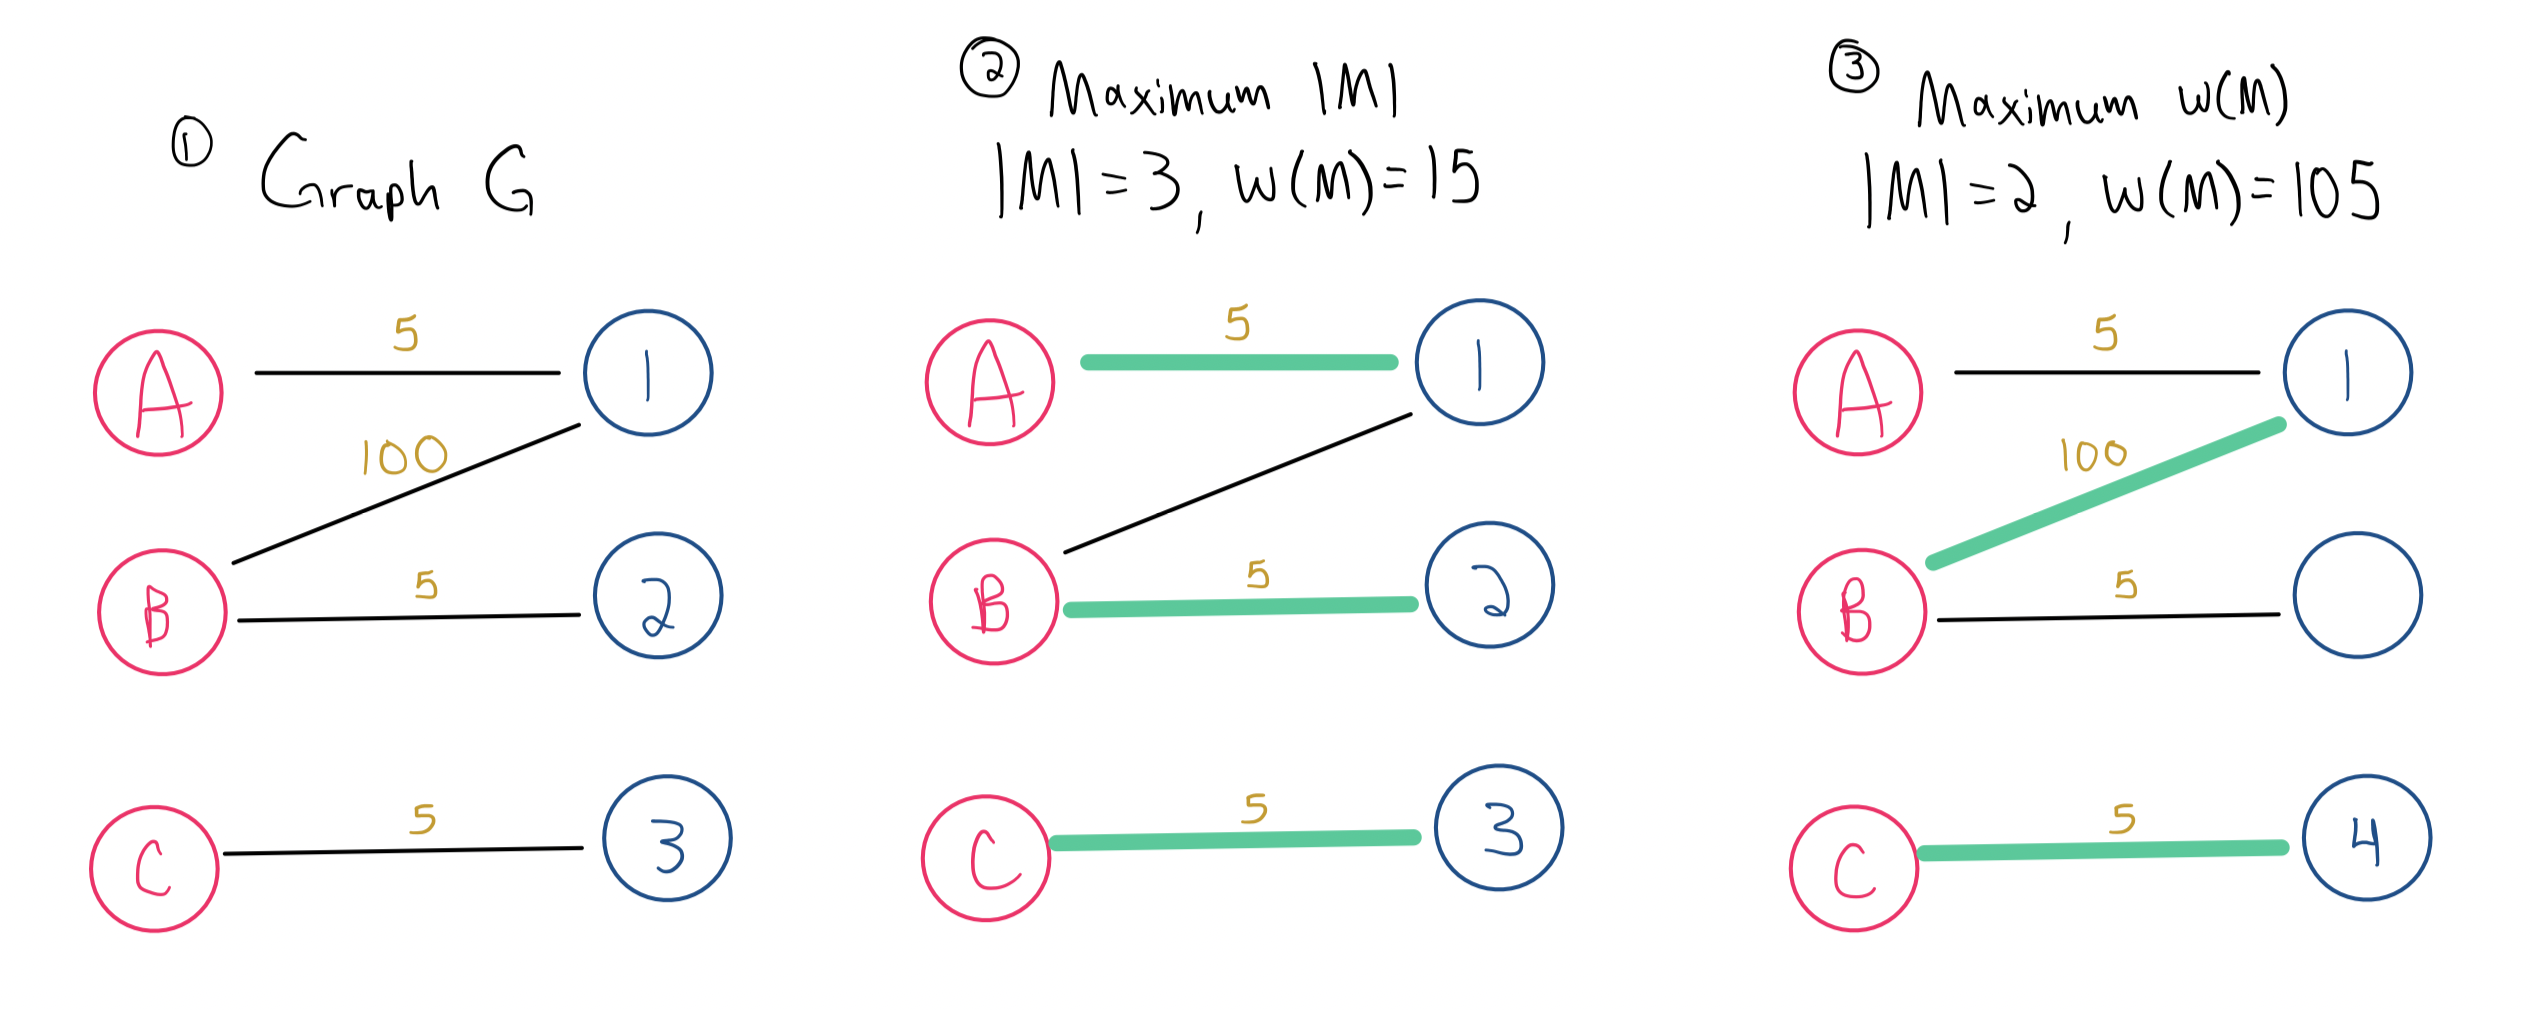
\includegraphics[scale=0.4]{photos/q4a.png}
        Consider the graph G drawn above composed of these inputs:
        \begin{itemize}
            \item Vertices: [A, B, C, 1, 2, 3]
            \item Edges: [(A, 1), (B, 1), (B, 2), (C, 3)]
            \item Weights: [5, 100, 5, 5]
        \end{itemize}
        In this graph, the maximum matching in (2) has size three, but the maximum weight matching in (3) has size two. Including the $(B, 1)$ edge thus yields a maximum weight matching at the cost of a maximum size matching.
   \end{quote} 

    \item (optional\footnotemark[1])
    One real-life constraint in kidney exchange is that donors $d$ are often associated with a particular patient $p$ (e.g. a close family member) such that $d$ is only willing to donate a kidney if $p$ receives a kidney from someone.  ($d$ would donate their kidney directly to $p$ if they could, but they are incompatible.) 
    Suppose we have an (unweighted) bipartite graph $G=(V_0\cup V_1,E)$ representing $n$ such donor-patient pairs, i.e. $V_0=\{d_0,d_1,\ldots,d_{n-1}\}$, $V_1 = \{p_0,p_1,\ldots,p_{n-1}\}$, where $p_i$ is the patient associated with donor $d_i$. We assume $\{d_i,p_i\}\notin E$ for each $i$.   Our goal is to find a matching $M$ of the largest possible size $|M|$, subject to the constraint that $d_i$ is matched in $M$ only if $p_i$ is matched in $M$. 

    Show that we can reduce this constrained version of the maximum matching problem to finding a maximum-weight {\em perfect} matching in an appropriate edge-weighted bipartite graph, where
    a perfect matching is a matching that matches all the vertices in the graph. (Hint: add edges $\{d_i,p_i\}$ with appropriate edge weights.) 
    \end{enumerate}

\end{enumerate}
\end{document}
